\documentclass[11pt]{article}
\usepackage{fancybox,subfigure}
\usepackage{fancyvrb,framed,graphicx}
\usepackage[figure]{algorithm2e}
\hoffset -0.7in
\voffset -1in
\textheight 9.5in
\textwidth 6.5in
\parskip8pt
\renewcommand{\rmdefault}{phv} % Arial
\renewcommand{\sfdefault}{phv} % Arial
\pagestyle{empty}
\begin{document}

\section*{Project Abstract/Summary}
In neuroscience, the potential for large scale collaboration and data sharing is seriously undermined 
by concerns over the management and handling of personally 
identifiable information (PII) in neuroimagery data sets. 
In particular, HIPAA and HITECH rules mandate substantial measures 
for the preservation of subject privacy. For the researcher, whose focus is on the science, the 
management of information privacy is a wholly burdensome task. 
The vast potential for sharing and meta analysis of neuroimagery in research goes unful�lled 
for two reasons; (i) systematic sanitization is hampered by the dearth of tools to systematically 
expunge PII from DICOM images, and (ii) an established work�ow that integrates sanitization into 
the data sharing process remains conspicuously absent. 

This proposal seeks to address both of these challenges by augmenting an established and popular software framework for managing and sharing neuroimagery  -- the Extensible Neuroimaging Archive Toolkit (XNAT) -- with a toolset and integrated workflow for redaction of PII in  DICOM image files. 
The redaction process to be engaged by this effort differs from naive sanitization techniques in that it uses pseudonymous identi�ers in a Privacy Mapping Database to 
disambiguate between subjects without tracking their identities. 
This approach gives researchers the maximum power and flexibility in sharing neuroimagery datasets, while transparently coping with PII considerations in a standardized data curation process. 

The proposed redaction toolset complements the data curation and management tools within XNAT and folds neatly within existing XNAT operational workflows and lab processes.
The toolset and workflow adhere to the secure design principles of psychological acceptability and least privilege, promoting broad user adoption and ensuring subject confidentiality.
The sanitization process itself built upon principles of legal redaction and rules of evidence, providing heightened levels of assurance for scientists and investigators for HIPAA compliance.

The long term objectives of this project are to create a comprehensive and practical infrastructure for managing PII in neuroimagery datasets, and to relieve the burden of the investigator from the technical aspects of data sanitization and redcation.
In so doing, this effort will remove substantial obstacles to large-scale collaboration and data sharing in neuroscience.

\eject

\section{Project Narrative/Relevance}
In neuroscience, the potential for large scale collaboration and data sharing is seriously undermined 
by concerns over the management and handling of personally identifiable information (PII) in neuroimagery data sets. 
This proposal seeks to address this problem by augmenting the Extensible Neuroimaging Archive Toolkit (XNAT) with a toolset and integrated workflow for pseudonymous redaction of PII in 
DICOM image files. 
The approach adopted by this effort gives researchers the maximum power and flexibility in sharing neuroimagery datasets, while transparently coping with PII considerations in a standardized data curation process. 

\eject

\section*{Facilities and Resources}

{\bf Institute of Bioinformatics and Computational Biology, University of Tulsa} - The Institute of Bioinformatics and Computational Biology (IBCB) spans a collection of research topics that include the development of new tools to support data analysis for the life sciences, and computational models that simulate biological processes.  
Significant energies of IBCB faculty and students are devoted to neuroinformatics in support of a large scale research collaboration between member institutions of the Tulsa Research Quadrangle (TRQ) � Laureate Insitute for Brain Research (LIBR), The University of Tulsa, OU-Tulsa, and the Oklahoma Medical Research Foundation (OMRF).

Laboratory space will be dedicated to project software development and testing in the College of Engineering and Natural Science's Keplinger Hall at the University of Tulsa.
The lab will house the equipment and personnel needed to complete the project. 

\hskip-.23in{\bf Laureate Institute for Brain Research, Laureate Psychiatric Hospital and Clinic} - The Laureate Institute of Brain Research  (LIBR) is commencing longitudinal studies to discover the genetic basis of brain behavior.
LIBR resources include a 40,000 sq. ft. neuroimaging facility dedicated to research, and containing a GE 750 3 Tesla scanner with plans underway to acquire additional scanners.
LIBR presently has 34 full-time professional staff, 12 of whom hold doctoral degrees.

Drs.\ Jerzy Bodurka and Pat Bellgowan from LIBR will provide guidance and counsel on the development of the proposed solution from a neuroscientific and end-user perspective.
Both are intimately familiar with the full spectrum of neuroimaging data formats and with the user and operator requirements as they pertain to established workflow patterns for the acquisition, maintenance and sharing of neuroimagery.

\hskip-.23in{\bf Neuroinformatics Research Group, Washington University School of Medicine} - The Neuroinformatics Research Group (NRG) is focused on facilitating the integration, mining, and sharing of data from across the neuroscientific realm. 
The NRG has developed and maintains a number of open-source and open-access projects along these lines, including the Extensible Neuroimaging Archive Toolkit (XNAT). 
The NRG is part of the Neuroimaging Laboratory in the Mallinckrodt Institute of Radiology at the Washington University School of Medicine. It is also a member of the Biomedical Informatics Research Network (BIRN) and receive additional support from the Howard Hughes Medical Institute and the McDonnell Center for Higher Brain Function.

The XNAT platform developed by members of the NRG provides the underlying software framework for the proposed effort.
Software developers of the neuroimage redaction solution will interact with computer scientists, system developers and researchers in the NRG regularly to ensure a smooth and successful integration of the technology produced by the effort.
\eject

\section*{Personnel Justification}

{\bf John Hale, Ph.D.} - Professor of Computer Science and Lead Research Scholar, Institute of Bioinformatics and Computational Biology, University of Tulsa (Principal Investigator):
Dr.\ Hale will devote 11\% of his time during the academic year and one month effort during the summer to supervise the software development effort.
\eject

\section*{Specific Aims}

In neuroscience, the potential for large scale collaboration and data sharing is seriously undermined 
by concerns over the management and handling of personally 
identifiable information (PII) in neuroimagery data sets. 
In particular, HIPAA and HITECH rules mandate substantial measures 
for the preservation of subject privacy. For the researcher, whose focus is on the science, the 
management of information privacy is a wholly burdensome task. 

While multi-institutional collaborations and meta-analyses can make good use of sanitized 
datasets, the vast potential for sharing and meta analysis of neuroimagery in research goes unful�lled 
for two reasons; (i) systematic sanitization is hampered by the dearth of tools to systematically 
expunge PII from DICOM images, and (ii) an established work�ow that integrates sanitization into 
the data sharing process remains conspicuously absent. 

This proposal seeks to address both of these challenges by augmenting the Extensible Neuroimaging Archive Toolkit (XNAT) with a toolset and integrated workflow for redaction of PII in 
DICOM image files. 
The redaction process to be engaged by this effort differs from naive sanitization techniques in that it uses pseudonymous identi�ers in a Privacy Mapping Database to 
disambiguate between subjects without tracking their identities. 
This approach gives researchers the maximum power and flexibility in sharing neuroimagery datasets, while transparently coping with PII considerations in a standardized data curation process. 

The specific aims of this project are:

\begin{enumerate}
\item Completion of a comprehensive redaction toolset for DICOM images: Dicom images are embedded with both sensitive personal health information (PHI) and PII data.� Redaction of this information will be comprehensive across the varying DICOM fields utilized by the various imaging systems (e.g., GE, Seimens, and Phillips DICOM formats).
\item Construction of a Privacy Mapping Database: This database will map neuroimage datasets to pseudonymous subject identifiers, enabling large scale data sharing, while preserving subject privacy under HIPAA regulations.
\item Design and integration of a data curation/redaction workflow within XNAT: This aim will integrate the tools developed in aims 1 and 2 within an established neuroimage archival framework to enhance both security of the data and functional utility of the database for the neuroscientific community.
\end{enumerate}

The proposed redaction toolset complements the data curation and management tools within XNAT and folds neatly within existing XNAT operational workflows and lab processes.
The toolset and workflow adhere to the secure design principles of psychological acceptability and least privilege, promoting broad user adoption and ensuring subject confidentiality.
The sanitization process itself built upon principles of legal redaction and rules of evidence, providing heightened levels of assurance for scientists and investigators for HIPAA compliance.

The long term objectives of this project are to create a comprehensive and practical infrastructure for managing PII in neuroimagery datasets, and to relieve the burden of the investigator from the technical aspects of data sanitization and redcation.
In so doing, this effort will remove substantial obstacles to large-scale collaboration and data sharing in neuroscience.

 \eject
 
\section*{Background and Significance}

This section presents the dominant neuroimage repositories and archival frameworks, along with related efforts in data sanitization.
It offers a gap analysis of the technologies and tools presented, and discusses the impact of
closing these gaps with proposed effort.

\subsection*{Related Work}

Researchers make use of online repositories for neuroimages to share data and their analyses.
The promise held for these repositories to foster large collaborative endeavors remains immense, but is limited by concerns over the privacy of study subjects.
Tools exist to sanitize neuroimage datasets, e.g., eliminating PII from DICOM images, but even these suffer from problems that limit their utility in fostering large-scale data sharing and collaboration.

\subsubsection*{fMRIDC}
The fMRI Data Center is a repository for peer-reviewed neuroimages and related study data \cite{vanhorn01}.  
While no longer open for new data submissions, the subject privacy policy holds researchers responsible for santizing their own data prior to submission. 
The Data Center performs a scan of submissions to remove any potentially identifying data overlooked by the researchers.  
Researchers may also remove anatomical image volumes to prevent reconstruction of the subject's face; otherwise, the Data Center will strip the images before they are made available.

This approach adequately protects the privacy of the subject but requires the researcher to maintain a list of subjects identifiers if necessary.  
It also has the potential to strip data it determines to be uniquely identifying without notifying the researcher.  
This prevents the researcher from reusing the identifier if the subject participates in a future imaging session.

\subsubsection*{XNAT (Extensible Neuroimaging Archive Toolkit)}
The Extensible Neuroimaging Archive Toolkit (XNAT) is an open software framework  that provides data management and control for neuroimaging studies \cite{xnat}.  
As such, XNAT is designed to facilitate multi-institutional research collaboration through data management and control.  
Data flows through XNAT in five phases: Data Acquisition, Quarantine, Local Use, Collaboration, and Public Access.  
In the Data Acquisition phase, data is uploaded to XNAT and is quarantined, where the user validates it before viewing and analyzing it.  
Users can then create subsets of the data that can be sent to collaborators or released for public viewing.

The XNAT platform consists of three architectural layers; a data archive, a user interface (including the standard web interface as well as desktop tools),  and a middleware engine.
XNAT uses XML to interface with existing neuroinformatics analysis tools and data repositories, underscoring the possibility of a federated solution for highly integrated collaborative research.  
XML allows implementations to extend the core XML schema for maximum customization, and supports easy translation between formats.

In its current state, XNAT provides basic support for sanitizing patient data.  
Investigators must perform this step manually using the DicomBrowser tool, which allows users to view or edit imaging session metadata.  
It is offered in both a graphical and command-line interface.  

The flexibility of XNAT allows researchers to upload data in multiple formats with varying study parameters; however, this presents a challenge when standardizing a sanitization process, requiring the end user to tailor the anonymization process to a particular study or session through anonymization scripts.  
Anonymization scripts are based on the DICOM tag key-value pairs.  
The language allows specification of operations to be performed on the attribute pairs and constraints by which the operations are applied.  
Allowed operations are assignment to set a default value for the attribute and deletion.
% TODO: Does this previous sentense make sense?


\subsubsection*{LONI De-identification Debablet}
The LONI De-identification Debablet is a software tool capable of reading medical images in a variety of formats and stripping them of an personally identifying information \cite{neu05}.
This tool is built on top of the LONI Debabeler execution engine, which facilitates translations between DICOM, ANALYZE, MINC and other medical image formats.
 
The De-identification Debablet It replaces a subject identifier with a user-defined identifier to permit anonymize tracking of datasets across subject populations.  
While it successfully de-identifies the images, this technique is suitable for localized use only; no solution is provided for decentralized neuroimage dataset tracking and management.   % TODO: Should this be centralized?
Thus, a researcher must define, manage and maintain identifying links between original and sanitized images.
The principal limitation herein is that this approach has no inherent method for identifying returning subjects or for recognizing datasets from the same subject. 

Additional complications in dataset sharing and management are encumbered by this scheme.
There may be other identifying features that an investigator wishes to alter or include, depending on the nature of the study and the sensitivity of the information.  
The investigator may also desire a more robust solution with expanded auditing capabilities to track the removal of data and to allow other authorized collaborators access to it.  
%For example, if Alice and Bob both want to add imaging sessions for Subject A, Alice must de-identify the data using an identifier that she defines.
%She must then communicate this identifier to Bob, who must also de-identify the scan he performs, specifying the same identifier that Alice has used.  
%While the De-identification debablet satisfactorily sanitizes the images, it requires manual maintenance of identifiers, which can be extremely cumbersome when used by multiple researchers.

\subsection*{Significance of Proposed Effort}
The proposed solution satifies HIPAA requirements regarding subject privacy while maintaining ease of use for the researcher.  
We offer an automated approach to redacting patient data for use with XNAT as a neuroimage repository.  
This project has two primary advantages over existing measures: (1) it provides a privacy map for linking and managing redacted identifiers across institutional boundaries, and (2) it is part of the XNAT processing pipeline and thus a natural part of collaborative workflow. 

Our solution seamlessly creates a privilege map of redacted subject data, creating pseudonymous identifiers to associate with subject datasets.  
%In the previous example, both Alice and Bob could upload their respective sessions with a single subject, and the system would verify that they both have access to the privacy map, then it would fully redact Bob's scan with the same information and settings that Alice has used.  
%A third user, Charlie, could then be given access to the all of the subject's redacted clinical data and images, which have an identifier that only Alice or Bob could link to the original subject.  
Cross-linking and validation of these new identifiers is managed systematically by middleware, and integrated transparently into the data curation and resource sharing workflows.
This permits persistent identifiers which, although they cannot be used to uniquely determine an individual's identity,  can be used to track the datasets associated with an individual (anonymous) subject. 

The primary responsibility for ensuring patient privacy still lies with the researcher, but the proposed solution minimizes the effort involved while enhancing the quality and utility of subject data.  
By integrating redaction within collaborative workflow, privacy management becomes a more systematic and intuitive process.


\section*{Preliminary Studies}
This effort builds upon the investigators and associated personnel�s experience in security compliance (HIPAA/HITECH), research data flow, and digital forensics. A background in all these areas provides the cross-discipline foundation for this effort to succeed.  

\subsection{Data Management and Compliance}
At the Laureate Institute for Brain Research, HIPAA compliance has typically been handled by the parent hospital system, however incorporating the neuroimaging component has shifted organizational boundaries, creating a new institute responsible for all IT and compliance aspects of the longitudinal study and associated research projects.  In the course of the institutional creation, a comprehensive examination of research data flows and compliance measures has been taken, paying close attention to the needs of core researchers and the nature of their external collaborations. 

This review revealed that scientific personnel use haphazard methods for data management, often relying on arcane naming systems and individualized workflows. As a new institution, with a shared information infrastructure, individualized flows prevent cross investigator collaboration. This barrier to growth mandated the need for centralized data management and analysis facilities\cite{drevets09}, with a tentative plan to build upon the XNAT architecture \cite{barclay09b} \cite{xnat}.

All personnel are trained in the theory of HIPAA compliance for research subjects, however there is a disconnect between what a researcher sees presented from his tools on screen to what is hidden in file metadata. This abstraction of PHI leads to data breeches of well meaning staff. This problem is not restricted to DICOM files; it is a bigger problem when sending datasets over physical media, where PHI can hide in low-level file system structures, file system meta-data, and operating system indices\cite{gavin paper}.

HIPAA regulations and supporting documents were designed for clinical care and the assumption of well-regulated centralized storage and access control.  This model is typically not used in dispersed neuroimaging studies where each researcher requires access to raw imaging data.  However, in this model data security compliance is almost impossible. Under HIPAA; PHI data must be protected by certain mechanisms, in ways often unknown and impractical for individual researchers \cite{nisthipaa}.

By using workflow tools such as the XNAT framework, an institution can more easily meet the HIPAA data security requirement, and by performing redaction against the centralized storage an organization complies with the privacy regulations as well \cite{nistpii}. 

XNAT is the leading candidate framework within which to embed a comprehensive digital redaction solution, due to the data management facilities and previous experience.

Recently, the PI led a team (with cooperation from the Neuroinformatics Research Group at the Washington University School of Medicine) that conducted an information security risk assessment for XNAT, yielding a deeper understanding of threats to and vulnerabilities in the platform \cite{schimke09}.

This afforded student developers and graduate students, who would implement this proposal, the opportunity to become familiar with the design and operation of XNAT. The risk assessment therefore provided an excellent basis on which to define operational and security requirements for an integrated digital redaction solution.

\subsection{Redaction}

Redaction is the process of removing privileged information from a document or set of documents before its presentation to other parties.  This is not a trivial process, in that redaction must include the entirety of targeted data to be removed, be scientifically sound, and provide verification to combat legal opposition to production data.

When a group from the University of Tulsa (including the PI) started addressing redaction for legal production in 2005, the recommendation from the NSA was to copy files to remove metadata\cite{nsaredact}. This approach was seen as crude since it was not scalable for many files, nor did it map the original data to the redacted version or provide any verification mechanisms. Borrowing techniques from cryptography, digital forensics, and operating system design, a redaction method was developed that (1) examined the data at different abstraction layers of the file/media, (2) created a mapping of redacted content to original, and (3) verified redaction of data \cite{redactieee} \cite{Barclay2007} \cite{redaction3}.

This above project was developed as a general framework for redaction, allowing the inclusion of domain and file type specific information to increase completeness.  The partnership with LIBR and this proposal will provide a test bed to adapt a limited version of the previous effort. There are eighteen PHI identifiers, which provide context when searching data; this computationally simple search space reduces complexity of proposed redaction engine code.

This proposal is built upon comments received at the 2009 USENIX security conference, where a poster was presented which explored the issue of comprehensive neuroimage redaction. Feedback reduced the scope of this proposal, concentrating on the DICOM layer first, with redaction of the full file system stack as a later target \cite{Barclay2009}.  

The cross institution nature of this effort provides an ideal setting for the development of an integrated neuroredaction solution. The cross discipline makeup and experience of computer security professionals, information technology managers, and neuroimagers enable a tailored redaction solution developed to address ease of use, compliance, and of confidentiality of all stakeholders.


\eject

\section*{Research Design and Methods}
\subsection*{Workflow}
The XNAT workflow is defined as the main sequence in \ref{fig:workflow}\cite{xnat}, our redaction process integrates into the XNAT framework by the provided pipeline feature.

This change is not exposed to the user, and the workflow process begins as normal at acquistion time. It is only after raw data is collected and stored according to the institution's local policy and is released from quarantine, that the option to redact data is provided.

\begin{figure}[hbt]
       \center{\includegraphics[scale=1]{workflow_pipeline.png}}
        \caption{\label{fig:workflow} Neuroimage redaction process workflow as experianced by the end users (modification in bold)}
\end{figure}

%what user sees
To redact the data the user manually initiates the redaction process which starts the redaction pipeline. The output of this pipeline is that redacted data is tagged and inputed into the system as new data. Being treated as new data, it follows normal XNAT workflow and is quarantined again, mandating a secondary sanity check before being being part of the normal XNAT mechanisms, this time under an privacy mapped user id. This privacy mapped data is used as normal data, being available for analysis and sharing with no modifications to XNAT itself.

%user choice
Specific information from the original DICOM file may be desirable, and needed, to be exported along with the redacted dataset. In this case, user defined options can keep embedded subject data (such as age, weight) in the resultant DICOM dataset. It is the duty of investigator to ensure multiple remote datasets aren't shared to the same entity and combined if that would violate privacy compliance. A privacy map naming scheme will be provided to counter this threat\cite{ohm}. 

%can't figure out a nice transition from userflow to dataflow
While the user workflow and interface to XNAT remains unchanged, there are some loosely coupled extensions to XNAT which allow redaction to occur. In \ref{fig:dataworkflow}, a logical view of the data path is presented. 

\begin{figure}[hbt]
       \center{\includegraphics[scale=1]{data_workflow.png}}
        \caption{\label{fig:dataworkflow} XNAT and Redaction Data Path (modifications in bold)}
\end{figure}

This data path is a supported extension to the XNAT framework, designed to allow additional features. In practice, XNAT calls an external program, like ours, which will be running on the same computer to manipulate data and communicate back to the XNAT. During this process, a copy of the data is made for the redaction engine, from which DICOM sanitization and verification occurs and original personally identifiable information is preserved in the privacy map. From here, the cleaned DICOM file are fed back into the XNAT similar to original acquisition.

% Do we need this part? Not sure if this hurts us or not. I think it's important since otherwise why have a privacy map, we need to expose this data is some manner.
The privacy map is not exposed to the user from XNAT, and due to the sensitive nature of contained data will only be available to administrators using a command line tool/API if integration of redacted information needs to be made available. 

% Sept 11 AB Changed process workflow picture to new architecture
% Sept 11 AB Seperated Data workflow to new picture represening pipline architecute

\subsection*{Implementation Architecture}

The XNAT platform is an integrated suite of software based on open source technologies and custom code. The software design is standard and expandable separating out client interfaces, middleware engines, and data archiving. This modular design eases development by having well formed boundaries, a tested core foundation, and debugging access to every area. An abstracted XNAT architecture is presented in \ref{fig:architecture} \cite{xnat}, with the redaction plug-in indicated in bold.

\begin{figure}[hbt]
       \center{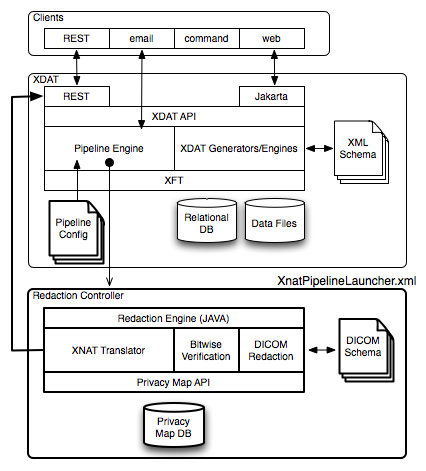
\includegraphics[scale=.7]{architecture_pipeline.png.png}}
        \caption{\label{fig:architecture} Preliminary architecture diagram (modifications in bold)}
\end{figure}
% Sept 11 AB - Changed pic to new architecture, PNG, no bounding box/export full size

The redaction effort can be divided logically and by software implementation into three primary components: (1) the redaction engine, (2) the privacy mapping database, and (3) the XNAT translator. The first two integrate into the XNAT pipeline facility\cite{xnatpipeline}, where the specification and configuration for the pipeline are defined in Extensible Markup Language (XML) files \cite{bray2000}. The XML documents are configuration files; which define how the pipeline works, and operates as a template for XNAT database and web presentation. The pipeline configuration and provided utility program enable the redaction process to be XNAT aware by providing feedback to the user via e-mail with problems or status updates.

The redaction engine is an expandable entry point and controller of the redaction tool, and by design has to start as a JAVA program. This is currently planned to encompass both the DICOM redaction procedure and the low-level bitwise verification mechanism, however final language choice and detailed design decisions will occur during development. 

The DICOM redaction component is based on in-depth knowledge of the DICOM file format and the conformance statements from the major MRI vendors. By parsing the DICOM file, a list of the name:value pairs can be extracted from the file itself. These defined duples identify PII, which can then be remapped to anonymized identifiers. This process of matching and replacement of name:value pairs enables the researcher to redact any DICOM field through the use of DICOM translation schemas. The shipping configuration will be tailored to HIPAA compliance, but the framework will be in place for any DICOM conversion. 

This remapping process is verified on the resultant DICOM image to ensure confidentiality of the original data. Digital forensics has pioneered the concept of ignoring the structure of files and file systems, opting instead to use low level bitwise datastream from disk and manually searching for information. This technique will be applied to DICOM files, searching for PII as search terms. This will be built on an open source data carving tool, such as scapel\cite{scapel}.

The anonymized identifiers and original data are stored in an encrypted privacy mapped database. This database is an integral part of the system, containing the link between the original images and their redacted counterparts. The API acts as a gatekeeper ensuring integrity of the databases by exposing a non-harmful subset of commands to the redaction engine and client application. The privacy map provides consistency between research subjects, ensuring the consistency of redacted ID to subject PII, preventing skew in statistical analysis due to duplication of data. This will be implemented as an additional database on top of the PostgreSQL instance already being utilized by XNAT. 

The last part of the redaction process is creation of new XNAT identifiers and transmission of the redacted data. The translator will communicate with XNAT through the HTTP REST interface provided \cite{fielding2000} and secure FTP where it will be uploaded to XNAT as new images, but with different metadata, where it will be processed as any incoming data. 

The proposed architecture is not complex, it is an extension to well conceived and executed system. The redaction design mimics that of XNAT itself; modular components, open source, simple to use, and simple to extend for future needs. 

\subsection*{Advantages over Current Solutions}

%The proposed effort has two primary objectives: (1) it provides a privacy map for linking and managing redacted identifiers across institutional boundaries, and (2) it is part of the pre-processing pipeline and can be invoked at the same time as the upload functionality. 

The proposed effort has three primary advantages over current tools and methodologies: (1) it provides a privacy map for linking and managing redacted identifiers across institutional boundaries, (2) it is part of the XNAT processing pipeline, leveraging the existing framework and interface, (3) unencumbered redaction building block, and lastly provide (4) verifiable redaction. 

The primary benefit of the privacy map is apparent; it automatically assigns a redacted identifier to subject record and removes potentially identifable information. This relieves the researcher of the burden of maintaining the subject's new identifier throughout a study.

The secondary benefit of the privacy map is that there is persistence in the sanitized identifier,  allowing multiple sessions over multiple researchers to be tracked without the need for manual maintenance. This fixes a huge problem with large transient data sets, adding consistency by not counting subjects twice.

Researchers will not have to maintain multiple data sets, their interface to data is mediated though XNAT, where the original image and a redacted image are centrally managed, and collaboration is facilitated.

Project code will be freely available and open source on a web site for others to extend, modify and freely distribute. The license will be an open source BSD style license, acting as a catalyst for innovation and development of a more complete redaction system.

Redaction will be performed and forensically verified to ensure confidentially of subject data. This technique is accepted for handling digital evidence, providing researchers legally accepted protection, and assurance that shared subject data does not fall under the breech notification requirements of HIPAA/HITECH.

\subsection*{Potential Challenges}

Because this project focuses on redacting PII meta-data from DICOM files, we are only considering one layer in the data stack.
This leaves redaction unresolved at the hard drive and file system levels, though with proper physical access controls to data centers and personal computers, the potential of a breach at this level is less immediate than at the logical DICOM level.
Since we are focusing on the DICOM layer, though it is desirable to be able to redact data from other formats as well.
The system will be flexible enough that future revisions can include other image formats.
There is also concern over the possibility that a subject's full facial image can be reconstructed from a sufficient amount of structural data; we do not attempt to address this in our proposed effort.

Though this project will reduce the effort required for redaction, the ultimate responsibility for redaction still lies in the hands of the researcher.
It is still possible to upload an unredacted data set to the XNAT repository and share it.
This risk can be reduced by the use of default redaction profiles to automatically de-identify any data set uploaded through the user interface.
Proper training and policy enforcement can reduce the likelihood of an accidental breach of privacy.

\subsection*{Timetable}

\eject
\bibliographystyle{plain}
\nocite{*}
\bibliography{NIHR03}
\end{document}